\documentclass[a4paper,11pt]{ctexart}
% 必须使用 XeLaTeX 编译器编译

\usepackage{geometry}
\usepackage{amsmath}
\usepackage{amssymb}
\usepackage{graphicx}
\usepackage{enumitem}
\usepackage{tikz}
\usepackage{tcolorbox} % 【核心】用于生成漂亮的边框

% --- 新增/修改部分 ---
% 1. 引入 hyperref 宏包以支持目录跳转，hidelinks 去除红框
\usepackage[hidelinks]{hyperref} 

% 2. 页面设置
\geometry{a4paper, scale=0.8}

% 3. 自定义一个命令 \mysection
% 作用：既保持 \section* 的无自动编号外观，又将其加入目录和 PDF 书签
\newcommand{\mysection}[1]{%
    \phantomsection % 创建锚点，让目录点击跳转准确
    \addcontentsline{toc}{section}{#1}% 将标题加入目录
    \section*{#1}% 显示标题
}

\title{通信原理-做过的习题整理}
\date{\today}
\author{}

\begin{document}

\maketitle

% 生成目录
\tableofcontents
\newpage % 目录后换页

% --- 正文开始 ---

\mysection{第一章}

\begin{enumerate}[label=\textbf{1-\arabic*}]
    \item 已知英文字母 $e$ 出现的概率为 $0.105$，$x$ 出现的概率为 $0.002$，试求 $e$ 和 $x$ 的信息量。
    \vspace{4em}

    \item 设有四个符号，其中前三个符号的出现概率分别为 $1/4, 1/8, 1/8$，且各符号的出现是相互独立的。试计算该符号集的平均信息量。
    \vspace{4em}

    \item[1-7] 某信源符号集由 A, B, C, D 和 E 组成，设每一符号独立出现，其出现概率分别为 $1/4, 1/8, 1/8, 3/16$ 和 $5/16$。若每秒传输 1000 个符号，试求：
    \begin{enumerate}
        \item 该信源符号的平均信息量；
        \item 1h 内传送的平均信息量；
        \item 若信源等概率发送每个符号，求 1h 传送的信息量。
    \end{enumerate}
    \vspace{4em}
    
\end{enumerate}

\noindent\textbf{【思考题】}
\begin{itemize}
    \item[1.] 深入分析全球 6G 愿景 (IMT-2030 六大愿景) 及各项性能指标要求，以及典型用例。
    \item[2.] 感知与通信的融合是 6G 的一大愿景，旨在让通信网络在传递信息的同时，还能感知物理环境，构建数字孪生世界。
\end{itemize}

\noindent\textbf{【思考题答案】}
\begin{itemize}
    \item[1.] 全球6G愿景（IMT-2030六大愿景）包括：沉浸式通信、超可靠低延迟通信、大规模连接、人工智能与通信的融合、感知与通信的融合、全球覆盖。性能指标要求：峰值速率达1Tbps，用户体验速率1Gbps，连接密度每平方公里千万级，时延0.1ms，可靠性99.99999\%，定位精度厘米级等。典型用例：全息通信、远程手术、自动驾驶、智能工厂、元宇宙、数字孪生等。
    \item[2.] 感知与通信的融合（ISAC）利用无线信号同时进行通信和环境感知，通过分析回波或信道状态信息实现高精度定位、手势识别、环境建模等。好处是节省硬件和频谱资源，挑战包括信号设计、干扰管理、算法复杂性、隐私安全等。应用场景有智能家居、智慧城市、交通监控、人体健康监测等。
\end{itemize}

\mysection{第四章}

\begin{enumerate}[label=\textbf{4-\arabic*}]
    \setcounter{enumi}{5} % 设置计数器，下一个将是 6
    \item 某个信息源由 A、B、C 和 D 等 4 个符号组成。设每个符号独立出现，其出现概率分别为 $1/4, 1/4, 3/16, 5/16$，经过信道传输后，每个符号正确接收的概率为 $1021/1024$，错为其它符号的条件概率 $P(x_i/y_j)$ 均为 $1/1024$，试求出该信道的容量 $C$ 等于多少比特/符号。
    \vspace{4em}
    
    \item 若上例中的 4 个符号分别用二进制码组 00、01、10、11 表示，每个二进制码元用宽度为 $0.5\text{ms}$ 的脉冲传输，试求出该信道的容量 $C_t$ 等于多少 b/s。
    \vspace{4em}
    
    \item 设一幅黑白数字相片有 $400$ 万个像素，每个像素有 $16$ 个亮度等级。若用 $3\text{kHz}$ 带宽的信道传输它，且信号噪声功率比等于 $20\text{dB}$，试问需要传输多少时间？
    \vspace{4em}
    
\end{enumerate}

\noindent\textbf{【思考题】}
\begin{itemize}
    \item 术语，模型，分类
    \item 无线信道的优缺点
    \item 信息传输速率计算、信道容量计算
\end{itemize}

\noindent\textbf{【思考题答案】}
    \begin{itemize}
        \item \textbf{术语、模型、分类}：
        \begin{itemize}
            \item \textbf{术语}：\textbf{消息}是信息的物理形式（如语音、图像）；\textbf{信息}是消息的有效内容（不确定性的消除）；\textbf{信号}是传输消息的载体（电或光信号）。
            \item \textbf{模型}：通信系统一般模型包括：信源 $\to$ 发送设备 $\to$ 信道（加噪声） $\to$ 接收设备 $\to$ 信宿。数字通信系统在此基础上增加了信源编译码、信道编译码、调制解调及同步模块。
            \item \textbf{分类}：按信号特征分为模拟通信和数字通信；按传输媒介分为有线通信和无线通信；按工作方式分为单工、半双工和全双工。
        \end{itemize}
        
        \item \textbf{无线信道的优缺点}：
        \begin{itemize}
            \item \textbf{优点}：无需架设物理线路，组网灵活，成本相对较低，支持移动通信，不受地形限制。
            \item \textbf{缺点}：信道特性不稳定（存在多径效应、阴影效应、衰落），易受电磁干扰，频谱资源有限，信号易被截获（保密性差）。
        \end{itemize}
        
        \item \textbf{信息传输速率计算、信道容量计算}：
        \begin{itemize}
            \item \textbf{信息速率与码元速率}：$R_b = R_B \log_2 M$，其中 $R_b$ 为比特率 (b/s)，$R_B$ 为波特率 (Baud)，$M$ 为进制数。
            \item \textbf{平均信息量（熵）}：$H(x) = -\sum_{i=1}^{M} P(x_i) \log_2 P(x_i)$ (bit/符号)。
            \item \textbf{香农公式（有噪信道极限）}：$C = B \log_2(1 + S/N)$ (b/s)，揭示了带宽 $B$ 和信噪比 $S/N$ 对信道容量的限制。
        \end{itemize}
    \end{itemize}

\mysection{第六章}
\vspace{1em}

\noindent \textbf{6-7} 已知码序列为 101100000000101，试确定相应的 AMI 码及 HDB$_3$ 码，并分别画出它们的波形图。

\vspace{4em} % 给 6-7 留出答题绘图空间

\noindent \textbf{6-11} 设基带传输系统的发送滤波器、信道及接收滤波器组成的总特性为 $H(\omega)$，若要求以 $2/T_B$ 波特的速率进行数据传输，验证图 P6-5 所示的各种 $H(\omega)$ 能否满足抽样点上无码间串扰的条件？

\begin{figure}[h]
\centering
\begin{tikzpicture}[>=stealth, scale=0.7]
    % --- 图(a) ---
    \begin{scope}[xshift=0cm]
        \draw[->] (-2.5,0) -- (2.5,0) node[right] {\small $\omega$};
        \draw[->] (0,0) -- (0,2.2) node[right] {\scriptsize $H(\omega)$};
        \draw[thick] (-1.2,0) -- (-1.2,1.6) -- (1.2,1.6) -- (1.2,0);
        \node[above left] at (0, 1.6) {\scriptsize 1};
        \node[right] at (1.2, 1.8) {\scriptsize 矩形};
        \node[below] at (-1.2,0) {\scriptsize $-\pi/T_B$};
        \node[below] at (0,0) {\scriptsize 0};
        \node[below] at (1.2,0) {\scriptsize $\pi/T_B$};
        \node at (0,-1.2) {\small (a)};
    \end{scope}

    % --- 图(b) ---
    \begin{scope}[xshift=8cm]
        \draw[->] (-3,0) -- (3,0) node[right] {\small $\omega$};
        \draw[->] (0,0) -- (0,2.2) node[right] {\scriptsize $H(\omega)$};
        \draw[thick] (-2,0) -- (-2,1.6) -- (2,1.6) -- (2,0);
        \node[above left] at (0, 1.6) {\scriptsize 1};
        \node[right] at (2, 1.8) {\scriptsize 矩形};
        \node[below] at (-2,0) {\scriptsize $-3\pi/T_B$};
        \node[below] at (0,0) {\scriptsize 0};
        \node[below] at (2,0) {\scriptsize $3\pi/T_B$};
        \node at (0,-1.2) {\small (b)};
    \end{scope}

    % --- 图(c) ---
    \begin{scope}[xshift=0cm, yshift=-4.5cm]
        \draw[->] (-3.5,0) -- (3.5,0) node[right] {\small $\omega$};
        \draw[->] (0,0) -- (0,2.2) node[right] {\scriptsize $H(\omega)$};
        \draw[thick] (-2.8,0) -- (0,1.6) -- (2.8,0);
        \node[above left] at (0, 1.6) {\scriptsize 1};
        \node[below] at (-2.8,0) {\scriptsize $-4\pi/T_B$};
        \node[below] at (0,0) {\scriptsize 0};
        \node[below] at (2.8,0) {\scriptsize $4\pi/T_B$};
        \node at (0,-1.2) {\small (c)};
    \end{scope}

    % --- 图(d) ---
    \begin{scope}[xshift=8cm, yshift=-4.5cm]
        \draw[->] (-3,0) -- (3,0) node[right] {\small $\omega$};
        \draw[->] (0,0) -- (0,2.2) node[right] {\scriptsize $H(\omega)$};
        \draw[thick, domain=-2.2:2.2, samples=100] plot (\x, {1.6*(1 + cos(\x*180/2.2))/2});
        \node[above left] at (0, 1.6) {\scriptsize 1};
        \node[right] at (1.2, 1.8) {\scriptsize 升余弦型};
        \node[below] at (-2.2,0) {\scriptsize $-2\pi/T_B$};
        \node[below] at (0,0) {\scriptsize 0};
        \node[below] at (2.2,0) {\scriptsize $2\pi/T_B$};
        \node at (0,-1.2) {\small (d)};
    \end{scope}
\end{tikzpicture}
\caption*{对应6-11}
\end{figure}

\vspace{4em}
    

\noindent \textbf{6-12} 欲以 $R_B = 10^3$ 波特的速率传输数字基带信号，试问采用图 P6-6 中的哪一种传输特性较好？并简要说明其理由。

\begin{figure}[h]
\centering
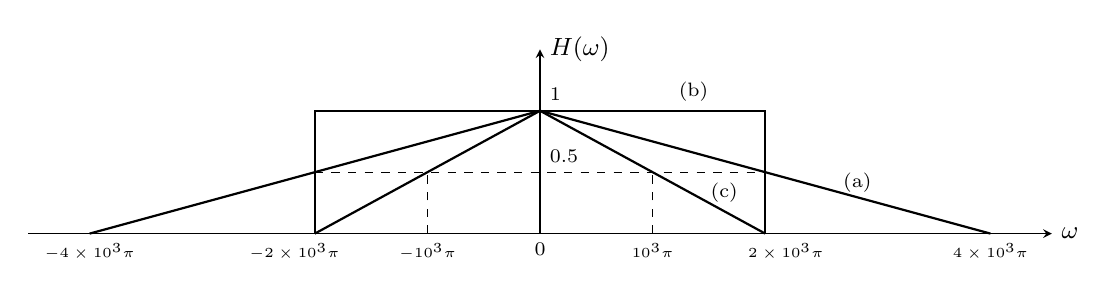
\begin{tikzpicture}[>=stealth, scale=1.3]
    % --- 坐标轴 ---
    \draw[->] (-5, 0) -- (5, 0) node[right] {\small $\omega$};
    \draw[->] (0, 0) -- (0, 1.8) node[right] {\small $H(\omega)$};

    % --- 垂直刻度 ---
    \node[above right] at (0, 1.2) {\scriptsize 1};
    \node[above right] at (0, 0.6) {\scriptsize 0.5};

    % --- 绘制曲线 ---
    % (b) 矩形
    \draw[thick] (-2.2, 0) -- (-2.2, 1.2) -- (2.2, 1.2) -- (2.2, 0);
    \node[above] at (1.5, 1.2) {\scriptsize (b)};

    % (a) 宽三角形
    \draw[thick] (-4.4, 0) -- (0, 1.2) -- (4.4, 0);
    \node at (3.1, 0.5) {\scriptsize (a)};

    % (c) 窄三角形
    \draw[thick] (-2.2, 0) -- (0, 1.2) -- (2.2, 0);
    \node at (1.8, 0.4) {\scriptsize (c)};

    % --- 辅助虚线 ---
    \draw[dashed] (-2.2, 0.6) -- (2.2, 0.6);
    \draw[dashed] (1.1, 0) -- (1.1, 0.6);
    \draw[dashed] (-1.1, 0) -- (-1.1, 0.6);
    \draw[dashed] (2.2, 0) -- (2.2, 0.6);
    \draw[dashed] (-2.2, 0) -- (-2.2, 0.6);

    % --- X轴标签 ---
    \node[below] at (0, 0) {\scriptsize 0};
    \node[below] at (1.1, 0) {\tiny $10^3\pi$};
    \node[below] at (2.4, 0) {\tiny $2 \times 10^3\pi$};
    \node[below] at (4.4, 0) {\tiny $4 \times 10^3\pi$};
    \node[below] at (-1.1, 0) {\tiny $-10^3\pi$};
    \node[below] at (-2.4, 0) {\tiny $-2 \times 10^3\pi$};
    \node[below] at (-4.4, 0) {\tiny $-4 \times 10^3\pi$};
\end{tikzpicture}
\caption*{对应6-12 图P6-6}
\end{figure}

\vspace{4em}
    

\noindent \textbf{【思考题】}

\begin{enumerate}
    \item 在数字基带系统中造成误码的原因是什么？请分析原因并给出减少误码的有效解决办法。
    \item 请画出第 IV 类部分响应系统组成框图。
\end{enumerate}

\vspace{2em}

\noindent \textbf{【思考题答案】}

\begin{enumerate}
    \item 在数字基带系统中造成误码的原因是什么？请分析原因并给出减少误码的有效解决办法。\\
    \textbf{答：} 
    \begin{itemize}
        \item \textbf{原因：} 
            \begin{enumerate}
                \item 噪声：信道中的加性高斯白噪声等；
                \item 码间串扰：由于信道不理想或带宽限制导致；
                \item 信道失真：频率选择性衰落、多径效应等；
                \item 同步误差：位同步、帧同步不准确；
                \item 判决门限漂移：接收机电路不稳定。
            \end{enumerate}
        \item \textbf{解决办法：}
            \begin{enumerate}
                \item 采用均衡技术（如时域均衡器）消除码间串扰；
                \item 选择抗干扰性强的传输码型（如HDB$_3$、AMI等）；
                \item 优化收发滤波器，满足奈奎斯特准则；
                \item 采用同步技术提高定时精度；
                \item 应用差错控制编码（如线性分组码、卷积码）和交织技术；
                \item 合理设计判决门限，采用自适应阈值。
            \end{enumerate}
    \end{itemize}

    \item 请画出第 IV 类部分响应系统组成框图。\\
    \textbf{答：} 第 IV 类部分响应系统框图如下：
    \begin{figure}[h]
        \centering
        \begin{tikzpicture}[>=stealth, node distance=1.5cm, auto]
            % 节点
            \node (input) {$a_k$};
            \node[draw, rectangle, right of=input] (precode) {预编码};
            \node[right of=precode] (bk) {$b_k$};
            \node[draw, rectangle, right of=bk] (delay) {$T_s$};
            \node[right of=delay] (bkm1) {$b_{k-1}$};
            \node[draw, circle, right of=bkm1] (sum) {$-$};
            \node[right of=sum] (ck) {$c_k$};
            \node[draw, rectangle, right of=ck] (mod) {$\mod 2$};
            \node[right of=mod] (output) {$\hat{a}_k$};
            % 连接
            \draw[->] (input) -- (precode);
            \draw[->] (precode) -- (bk);
            \draw[->] (bk) -- (delay);
            \draw[->] (delay) -- (bkm1);
            \draw[->] (bk) -- (sum);
            \draw[->] (bkm1) -- (sum);
            \draw[->] (sum) -- (ck);
            \draw[->] (ck) -- (mod);
            \draw[->] (mod) -- (output);
            % 标注
            \node[above of=precode, node distance=1cm] {差分编码};
            \node[above of=sum, node distance=1cm] {相关编码};
            \node[above of=mod, node distance=1cm] {模2判决};
        \end{tikzpicture}
        \caption{第 IV 类部分响应系统框图}
    \end{figure}
    其中，预编码（差分编码）规则：$b_k = a_k \oplus b_{k-1}$，相关编码：$c_k = b_k - b_{k-1}$，模2判决：$\hat{a}_k = c_k \mod 2$。
\end{enumerate}

\mysection{第七章}

\begin{enumerate}[label=\textbf{7-\arabic*}]
    \item 设发送的二进制信息序列为 1011001，码元速率为 2000 Baud，载波信号为 $\sin(8\pi \times 10^3 t)$。试确定：
    \begin{enumerate}
        \item 每个码元中包含多少个载波周期？
        \item 画出 OOK、2PSK 及 2DPSK 信号的波形，并注意观察其波形各有什么特点。
        \item 计算 2ASK、2PSK、2DPSK 信号的第一谱零点带宽。
    \end{enumerate}
    \vspace{4em}
    
    \item 设某 2FSK 调制系统的码元速率为 2000 Baud，已调信号的载频分别为 6000Hz (对应“1”码) 和 4000Hz (对应“0”码)。
    \begin{enumerate}
        \item 若发送的信息序列为 1011001，试画出 2FSK 信号的时间波形；
        \item 试画出 2FSK 信号的功率谱密度示意图，并计算 2FSK 信号的第一谱零点带宽。
        \item 讨论应选择什么解调方法解调该 2FSK 信号。
    \end{enumerate}
    \vspace{4em}
    
    \setcounter{enumi}{11} % 设置计数器
    \item 已知数字信息为“1”时，发送信号的功率为 $1\text{kW}$，信道损耗为 $60\text{dB}$，接收端解调器输入的噪声功率为 $10^{-4}\text{W}$，试求包络检波 OOK 和相干解调 2PSK 系统的误码率。
    \vspace{4em}
    
\end{enumerate}

\noindent\textbf{【思考题】}
\begin{enumerate}
    \item 试比较四种二进制数字调制系统的频带宽度、频带利用率和误码率。
    \item 二进制数字调制系统的误码率与哪些因素有关？如何提高系统的可靠性？
\end{enumerate}

\noindent\textbf{【思考题答案】}
\begin{enumerate}
    \item 四种二进制数字调制系统的比较：
        \begin{itemize}
            \item \textbf{频带宽度}：
                \begin{itemize}
                    \item 2ASK 和 2PSK（包括 2DPSK）：第一谱零点带宽为 $2R_B$，其中 $R_B$ 为码元速率。
                    \item 2FSK：带宽约为 $|f_1 - f_2| + 2R_B$，通常大于 2ASK 和 2PSK。
                \end{itemize}
            \item \textbf{频带利用率}（单位带宽传输的码元速率）：
                \begin{itemize}
                    \item 2ASK 和 2PSK：理论最大为 $1$ Baud/Hz，但实际由于需要带宽 $2R_B$，所以利用率约为 $0.5$ Baud/Hz。
                    \item 2FSK：由于带宽较宽，频带利用率较低，通常小于 $0.5$ Baud/Hz。
                \end{itemize}
            \item \textbf{误码率}（在相同信噪比条件下，从好到差排列）：
                \begin{itemize}
                    \item 相干解调 2PSK 误码率最低。
                    \item 相干解调 2DPSK（实际采用差分相干解调时，性能略差于相干 2PSK）。
                    \item 相干解调 2ASK 和 2FSK 误码率相近，但 2ASK 对门限敏感。
                    \item 非相干解调（包络检波）性能差于相干解调，其中非相干 2FSK 优于非相干 2ASK。
                \end{itemize}
        \end{itemize}

    \item 二进制数字调制系统的误码率主要与以下因素有关：
        \begin{itemize}
            \item \textbf{信噪比}：信噪比越高，误码率越低。
            \item \textbf{调制方式}：在相同信噪比下，2PSK 抗噪声性能最好，2FSK 次之，2ASK 最差。
            \item \textbf{解调方式}：相干解调比非相干解调性能好，但设备复杂。
            \item \textbf{信道特性}：如多径、衰落等会影响误码率。
            \item \textbf{码间串扰}：若带宽有限或传输特性不理想，会引起码间串扰，增加误码率。
        \end{itemize}
        提高系统可靠性的方法：
        \begin{itemize}
            \item 增加发送功率以提高信噪比。
            \item 选择抗噪声性能好的调制解调方式，如 2PSK 相干解调。
            \item 采用差错控制编码（信道编码）来检错和纠错。
            \item 改善信道特性，如采用均衡技术消除码间串扰。
            \item 采用分集技术、自适应技术等对抗衰落。
        \end{itemize}
\end{enumerate}

\mysection{第八章}
\noindent \textbf{8-1} 已知 4PSK 系统的传输速率为 $2400\,\text{b/s}$，试问：

\begin{enumerate}[label=(\arabic*)]
    \item 4PSK 信号的谱零点带宽和频带利用率 ($\text{b}/(\text{s}\cdot\text{Hz})$)；
    
    \item 若对基带信号采用 $\alpha = 0.4$ 余弦滚降滤波预处理，再进行 4PSK 调制，这时占用的信道带宽和频带利用率为多大？
    
    \item 若传输带宽不变，而比特率加倍，则调制方式应作何改变？
    
\end{enumerate}

\vspace{4em} % 题目间距

\noindent \textbf{8-2} 设发送数字序列为 $+1-1-1-1-1-1-1-1+1$，试画出相应的 MSK 信号相位变化图。若码元速率为 $1000\text{B}$，载频为 $3000\text{Hz}$，试画出此 MSK 信号的波形。
\vspace{4em}
    

\mysection{第九章}
% --- 题目 9-3 ---
\noindent \textbf{9-3} 设 2FSK 信号为
\begin{equation*}
    \begin{cases}
        s_0(t) = A\sin 2\pi f_0 t & 0 \leqslant t \leqslant T \\
        s_1(t) = A\sin 2\pi f_1 t & 0 \leqslant t \leqslant T
    \end{cases}
\end{equation*}
且 $f_0 = 2/T$，$f_1 = 2f_0$，$s_0(t)$ 和 $s_1(t)$ 等概出现。

\begin{enumerate}[label=(\arabic*)]
    \item 试画出其相关接收机原理框图；
    \item 设发送码元 010，试画出接收机各点时间波形；
    \item 设信道高斯白噪声的双边功率谱密度为 $n_0/2 \, (\text{W}/\text{Hz})$，试求该系统的误码率。
\end{enumerate}

\vspace{4em} % 题目间距

% --- 题目 9-6 ---
\noindent \textbf{9-6} 设二进制双极性信号最佳传输系统中，信号“0”和“1”是等概率发送的，信号传输速率为 $56\,\text{kb/s}$，接收码元波形为不归零矩形脉冲，信道加性高斯白噪声的双边功率谱密度等于 $10^{-15}\,\text{W}/\text{Hz}$。试问为使误码率不大于 $10^{-5}$，需要的最小接收信号功率等于多少？
\vspace{4em}
    
\mysection{第十章}

% --- 题目 10-10 ---
\noindent \textbf{10-10} 设输入信号抽样脉冲值为 $+635\Delta$（$\Delta$ 表示一个最小量化单位），采用 13 折线 A 律 PCM 编码。试确定：
\begin{enumerate}[label=(\arabic*)]
    \item 此时编码器输出码组、编码电平和量化误差；
    \item 对应于该 7 位码（不包括极性码）的均匀量化 11 位码；
    \item 译码电平和译码后的量化误差。
\end{enumerate}

\vspace{4em}

% --- 题目 10-11 ---
\noindent \textbf{10-11} 采用 13 折线 A 律编译码电路，设接收端译码器收到的码组为“01010011”，最小量化间隔为 1 个量化单位 ($\Delta$)。试求：
\begin{enumerate}[label=(\arabic*)]
    \item 译码器输出（按量化单位计算）；
    \item 相应的 12 位（不包括极性码）线性码（均匀量化）。
\end{enumerate}

\vspace{4em}

% --- 题目 10-17 ---
\noindent \textbf{10-17} 已知语音信号的最高频率 $f_H=3400\text{Hz}$，若用线性 PCM 系统传输，要求信号量化噪声比 $S/N_q$ 不低于 $30\text{dB}$。试求此 PCM 系统所需的奈奎斯特带宽。

\vspace{4em}

% --- 题目 10-18 ---
\noindent \textbf{10-18} 已知模拟信号 $f(t) = 10\sin(4000\pi t) + \sin(8000\pi t) \, (\text{V})$，对其进行 A 律 13 折线 PCM 编码。设一个输入抽样脉冲幅度为 $0.546875$ 伏，最小量化间隔为 1 个量化单位 ($\Delta$)。
\begin{enumerate}[label=(\arabic*)]
    \item 试求此时编码器的输出码组和量化误差；
    \item 若采用时分多路系统传输 10 路编码后的 PCM 信号，传输波形为非归零的矩形脉冲时，试确定该 PCM 时分多路信号的信息传输速率和传输带宽（第一零点带宽）。
\end{enumerate}
\vspace{4em}
    
\end{document}